\LTcapwidth=\textwidth

\setlength\aboverulesep{2pt}\setlength\belowrulesep{2pt}
\setlength\cmidrulekern{1pt}\setlength\cmidrulewidth{1pt}
\renewcommand\arraystretch{1.2}\setlength\tabcolsep{5pt}

\begin{longtable}{lll} 
\caption{Formulations and example response curves for a variety of indicator scoring methods that compare
observed values ($x_i$) to associated benchmark, thresholds or references values ($B_i$ and
dashed line). The Scaled Modified Amplitude Method can be viewed as three Steps: I. Initial Score
generation, II. Score capping (two alternatives are provided) and III. Scaling to the range
[0,1]. The first of the alternative capping formulations simply caps the Scores to set values (on a
$log_2$ scale), whereas the second formulation (Quantile based, where $Q1$ and $Q2$ are quantiles) allows thresholds quantiles to be used
for capping purposes.  Dotted lines represent capping boundaries.
In the Logistic Scaled Amplitude method, $T$ is a tuning parameter that controls the logistic rate (steepness at the inflection point).
For the purpose of example, the benchmark was set to 50.}\label{tab:indexMethods}\\[0em]
\toprule
\textbf{Method}&\textbf{Formulation}&\textbf{Response curve}\\
\midrule
\endfirsthead
\multicolumn{3}{l}{\textit{Table \ref{tab:indexMethods}: Report Card indexing methods, continued}}\\
\toprule
\textbf{Method}&\textbf{Formulation}&\textbf{Response curve}\\
\midrule
\endhead
\specialrule{1pt}{0pt}{0pt}
\endfoot
%%%%%%%%%%%%%%%%%%%%%%%%%%%%%%%%%%%%%%%%%%%%%%%%%%%%%%%%%%%%%%%%%%%%
\parbox[c][10em][t]{5em}{Binary\\compliance}&
\parbox[c][10em][t]{23em}{
\left$$
Score_i =
\left\{
\begin{array}{l l}
1 & \text{if}~x_i \le B_i\\
0 & \text{if}~x_i~\text{else}\\
\end{array}
$$
}
&
\parbox[c][10em][t]{10em}{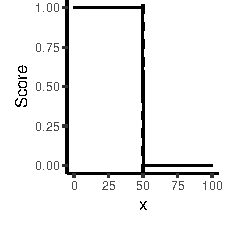
\includegraphics[]{figures/Indices/binary.pdf}}\\
\midrule
%%%%%%%%%%%%%%%%%%%%%%%%%%%%%%%%%%%%%%%%%%%%%%%%%%%%%%%%%%%%%%%%%%%%
\parbox[c][10em][t]{5em}{Benchmark and WCS}&
\parbox[c][10em][t]{23em}{
\left$$
Score_i =
\left\{
\begin{array}{l l}
100 & \text{if}~x_i \le B_i\\
0 & \text{if}~x_i \ge WCS_i\\
\left[1.0-\begin{vmatrix}\frac{x_i - B_i}{WCS_i - B_i}\end{vmatrix}\right].100 & \text{else}
\end{array}
$$
}
&
\parbox[c][10em][t]{10em}{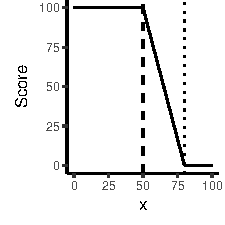
\includegraphics[]{figures/Indices/wcs.pdf}}
\\
\midrule
%%%%%%%%%%%%%%%%%%%%%%%%%%%%%%%%%%%%%%%%%%%%%%%%%%%%%%%%%%%%%%%%%%%%
\parbox[c][10em][t]{5em}{Amplitude}&
\parbox[c][10em][t]{23em}{
\left$$
Score_i = \left\{
\begin{array}{l l}
(\frac{x_i}{B_i})^{-1} & \text{if}>B_i=\text{fail}\\
(\frac{x_i}{B_i})^{1} & \text{if}<B_i=\text{fail}\\
\end{array}$\\[1em]
$Score_i = \frac{100\times Score_i}{1+Score_i}$
$$
}
&
\parbox[c][10em][t]{10em}{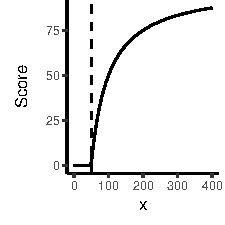
\includegraphics[]{figures/Indices/amp.pdf}}
\\
\midrule
%%%%%%%%%%%%%%%%%%%%%%%%%%%%%%%%%%%%%%%%%%%%%%%%%%%%%%%%%%%%%%%%%%%%
\parbox[c][10em][t]{5em}{Modified Amplitude}&
\parbox[c][10em][t]{23em}{
I. Raw (MAMP)\\
\left$$
Score_i = \left\{
\begin{array}{l l}
log_2(\frac{x_i}{B_i})^{-1} & \text{if}>B_i=\text{fail}\\
log_2(\frac{x_i}{B_i})^{1} & \text{if}<B_i=\text{fail}\\
\end{array}$
$$
}
&
\parbox[c][10em][t]{10em}{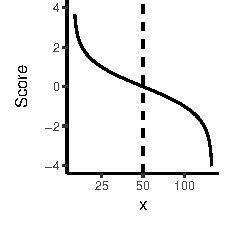
\includegraphics[]{figures/Indices/mamp.pdf}}\\
%%%%%%%%%%%%%%%%%%%%%%%%%%%%%%%%%%%%%%%%%%%%%%%%%%%%%%%%%%%%%%%%%%%%
\parbox[c][10em][t]{5em}{}&
\parbox[c][10em][t]{23em}{
II. Fixed caps (Fold=2; [0.5,2]) \textcolor{gray}{(Fold=4; [0.25,4])}\\
\left$$
Score_i = \left\{
\begin{array}{l l}
log_2(1/2) & \text{if}~Score_i < -1\\
log_2(2/1) & \text{if}~Score_i > 1\\
Score_i &otherwise\\
\end{array}$
$$
}
&
\parbox[c][10em][t]{10em}{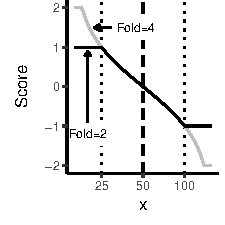
\includegraphics[]{figures/Indices/cmamp.pdf}}\\
%%%%%%%%%%%%%%%%%%%%%%%%%%%%%%%%%%%%%%%%%%%%%%%%%%%%%%%%%%%%%%%%%%%%


\parbox[c][10em][t]{5em}{}&
\parbox[c][10em][t]{23em}{
II. Quantile/extremes based caps ([15,170])\\
\left$$
Score_i = \left\{
\begin{array}{l l}
log_2(\frac{Q1}{B_i})^{-1} & \text{if}~x_i<Q1\\
log_2(\frac{Q2}{B_i})^{-1} & \text{if}~x_i>Q2\\
Score_i &otherwise\\
\end{array}$
$$
}
&
\parbox[c][10em][t]{10em}{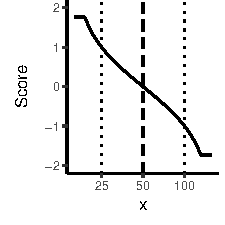
\includegraphics[]{figures/Indices/qmamp.pdf}}\\
%%%%%%%%%%%%%%%%%%%%%%%%%%%%%%%%%%%%%%%%%%%%%%%%%%%%%%%%%%%%%%%%%%%%
\parbox[c][10em][t]{5em}{}&
\parbox[c][10em][t]{23em}{
III. Scaled (Fixed: Fold=2)\\
$$
Score_i = \frac{Score_i - min(Score_i)}{max(Score_i) - min(Score_i)}
$$
}
&
\parbox[c][10em][t]{10em}{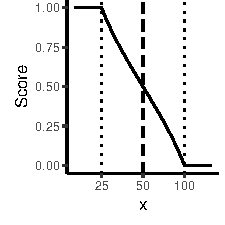
\includegraphics[]{figures/Indices/fsmamp.pdf}}\\
\midrule
%%%%%%%%%%%%%%%%%%%%%%%%%%%%%%%%%%%%%%%%%%%%%%%%%%%%%%%%%%%%%%%%%%%%
\parbox[c][10em][t]{5em}{Logistic Scaled Modified Amplitude}&
\parbox[c][10em][t]{23em}{
Raw\\
\left$$
Score_i = \left\{
\begin{array}{l l}
log_2(\frac{x_i}{B_i})^{-1} & \text{if}>B_i=\text{fail}\\
log_2(\frac{x_i}{B_i})^{1} & \text{if}<B_i=\text{fail}\\
\end{array}$\\
$Score_i = \frac{1}{1+e^{Score_i.-T}}$
$$
}
&
\parbox[c][10em][t]{10em}{\includegraphics[]{gigures/Indices/lsmamp.pdf}}\\
%%%%%%%%%%%%%%%%%%%%%%%%%%%%%%%%%%%%%%%%%%%%%%%%%%%%%%%%%%%%%%%%%%%%
\parbox[c][10em][t]{5em}{Logistic}&
\parbox[c][10em][t]{23em}{
Raw\\
\left$$
Score_i = \left\{
\begin{array}{l l}
\frac{1}{1+e^{T.(x_i/B_i)}}& \text{if}>B_i=\text{fail}\\
\frac{1}{1+e^{-T.(x_i/B_i)}}& \text{if}<B_i=\text{fail}\\
\end{array}$
$$
}
&
\parbox[c][10em][t]{10em}{\includegraphics[]{figures/Indices/lsmamp.pdf}}\\
\bottomrule
\end{longtable}